
\documentclass{article}

\usepackage{ amssymb }
\usepackage{ mathrsfs }
\usepackage{graphicx}

\setlength\parindent{0pt} % Removes all indentation from paragraphs


\begin{document}
\title{Physics Problems: \#1}

\author{For Lucas or Maria Camila}

\date{\today}
\maketitle


\section*{Problem Name$^1$}

Problem Description.\\

%To insert a figure
%\begin{figure}[h!]
%\begin{center}
%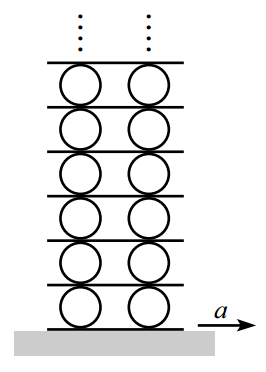
\includegraphics[width=0.3\textwidth]{tower.png}
%\end{center}
%\caption{Cylinder Tower.}
%\label{fig:tower}
%\end{figure}

\vspace{2mm}

\begin{center}
\noindent\rule{8cm}{0.4pt}\\
\end{center}

\noindent [1] Reference and link \texttt{https://www...}

\end{document}